\chapter{Problembeschreibung}

Das folgende Kapitel beschäftigt sich mit der Beschreibung der Problemstellung. Dazu wird zuerst das Ziel der Arbeit formuliert. Es folgen grundsätzliche Definitionen und die Beschreibung des zu bearbeitenden Datenbestandes. Abschließend wird die gewählte Lösungsstrategie konzeptionell beschrieben.

\section{Zielstellung}

Das Ziel dieser Arbeit besteht darin, aus vorhandenen Tag-Daten unter Zuhilfenahme von Integration anderer Daten Assoziationen zu extrahieren. Diese Beziehungen sollten im Optimalfall Zusammenhänge widerspiegeln, die zur Verbesserung der Benutzererfahrung beim Suchen nach bestimmten Themen, für Marketingmaßnahmen und generell für ein besseres Verständnis der auf einer Online-Plattform angebotenen Inhalte genutzt werden können.

Nutzbare Beziehungen können vielfältiger Art sein. Denkbar sind beispielsweise

\begin{itemize}
    \item inhaltliche Zusammenhänge, die mittels Clustering-Algorithmen später zu Themengebieten zusammengefasst werden
    \item Worthierarchien, aus denen Kategoriebäume erzeugt werden
    \item Wortformen, die dazu genutzt werden, mehrere Begriffe zusammenzufassen und somit mehr als nur eine wörtliche Suche zu ermöglichen
    \item Verknüpfungen von Wörtern, die über inhaltliche Zusammenhänge hinausgehen, beispielsweise Verbindungen Von Themengebieten mit bestimmten Emotionen, Produkten oder Personen
\end{itemize}

Ausgangsbasis für alle Überlegungen und Berechnungen sind die gesammelten Tag-Daten der Online-Plattform Spreadshirt, deren Struktur und Qualität im nächsten Abschnitt erläutert und diskutiert wird.

\section{Aufbau und Qualität der Daten}
\label{data}

Im folgenden Abschnitt sollen die intern bei Spreadshirt vorhandenen Datenquellen genannt und beschrieben werden. Außerdem wird der Umfang und die Qualität des Datenbestandes diskutiert.

\subsection{Tag-System}
\label{tag-system}

Ein Tag-System besteht im Allgemeinen aus den Mengen \(D\), \(T\) und \(U\). \(D\) bezeichnet die Menge der Dokumente. Ein Dokument \(d\) kann ein beliebiger Datensatz sein, beispielsweise ein Bild, Artikel oder Produkt. Die Menge \(U\) stellt alle Benutzer des Systems dar. Ein Benutzer \(u\) kann neben einem Index weitere Informationen besitzen, die jedoch hier im Kontext des Tag-Systems nicht tiefer gehend behandelt werden. \(T\) ist die Menge der Tags. Ein Tag \(t\) ist eine beliebige Zeichenkette. \(T\) bildet also das \emph{Vokabular} des Tag-Systems.

Die Benutzer können beliebige Dokumente mit beliebigen Tags versehen. Der Vorgang des \emph{Taggens} kann also durch die Relation \(R = D \times U \times T\) beschrieben werden, welche Tupel der Form \((d, u, t)\) enthält.

Der Betreiber der Online-Plattform kann bestimmte Aspekte des Tag-Systems begrenzen. Können alle Benutzer beliebige Tags an beliebigen Dokumente vergeben, spricht man von einer \emph{Folksonomy} \cite{ip2009}.

\begin{figure}
\label{fig:tagsystem}
\begin{center}
    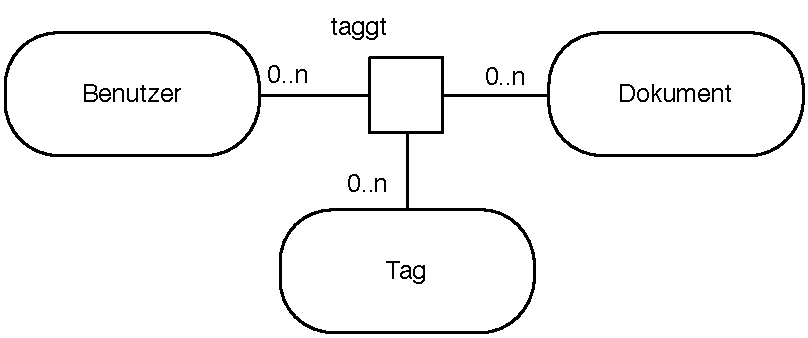
\includegraphics[width=0.6\textwidth]{tag_system}
\end{center}
\caption{Tag-System als Entity-Relationship-Diagramm}
\end{figure}


Im Fall von Spreadshirt ist die Vergabe von Tags auf die Menge der Partner \(P \subseteq U\) begrenzt (siehe auch \ref{spreadshirt}). Die Dokumente, die von den Partnern getaggt werden können, sind auf die Designs und Artikel beschränkt, die der Partner selbst angelegt hat. Eine Beschreibung kann also ausschließlich durch den Autor des Inhaltes erfolgen. Deshalb fehlt im Vergleich zu anderen Tag-Systemen auch die Information, welcher Benutzer den Tag vergeben hat.

Des Weiteren besitzen Tags in der Spreadshirt-Datenbank ein Attribut \emph{Sprache} aus der Menge \(L\). Die Sprache spielt bei der Eingabe und Anzeige der Tags zu Dokumenten eine Rolle. Je nach eingestellter Sprache auf der Webseite erstellt und sieht der Benutzer nur Tags, die mit dieser Sprache markiert sind.

Zum Zeitpunkt der Bearbeitung dieser Arbeit befanden sich in der Datenbank der europäischen Spreadshirt-Plattform:

\begin{itemize}
    \item \num{2072079} Tags
    \item \num{6433410} Benutzer
    \item \num{26147860} Dokumente (\num{16494430} Artikel und \num{9653430} Designs)
    \item \num{76978414} Taggings
\end{itemize}

In der Menge der Tags befinden sich Tags in \num{15} verschiedenen Sprachen. Es wurden insgesamt \num{71936424} Dokumente mit Tags versehen.

\subsection{Clicktracking}
Spreadshirt betreibt ein Clicktracking-System. Dieses System dient dazu, aufzuzeichnen, welche Artikel auf Suchergebnisseiten von Benutzern angeklickt werden. Dabei ist unerheblich, ob der Benutzer bei Spreadshirt registriert und angemeldet ist. Dieses System sammelt Daten von beiden Spreadshirt-Plattformen (siehe \ref{platforms}) und erzeugt bei jedem Klick eines Besuchers auf ein Suchergebnis einen Datensatz mit folgenden Attributen:

\begin{itemize}
    \item Suchbegriff
    \item Plattform, \emph{EU} oder \emph{NA}
    \item Zeitstempel des Klicks
    \item ID des geklickten Dokumentes
    \item Position des geklickten Dokumentes auf der Ergebnisseite
    \item Sprache
\end{itemize}

Die Nutzung der Clicktracking-Daten liefert eine andere Sicht auf die Metadaten der Produkte als die Tags. Die Klicks liefern eine Einschätzung des suchenden Benutzers, ob die Metadaten, die für den Suchindex verwendet werden, zum Artikel selbst passen. Die Grundannahme ist hierbei, dass Benutzer nur auf Suchergebnisse klicken, die ihren Erwartungen bezüglich des Suchbegriffes gerecht werden. Abbildung \ref{fig:search_result} zeigt ein Beispiel für ein Suchergebnis.

\begin{figure}
\centering
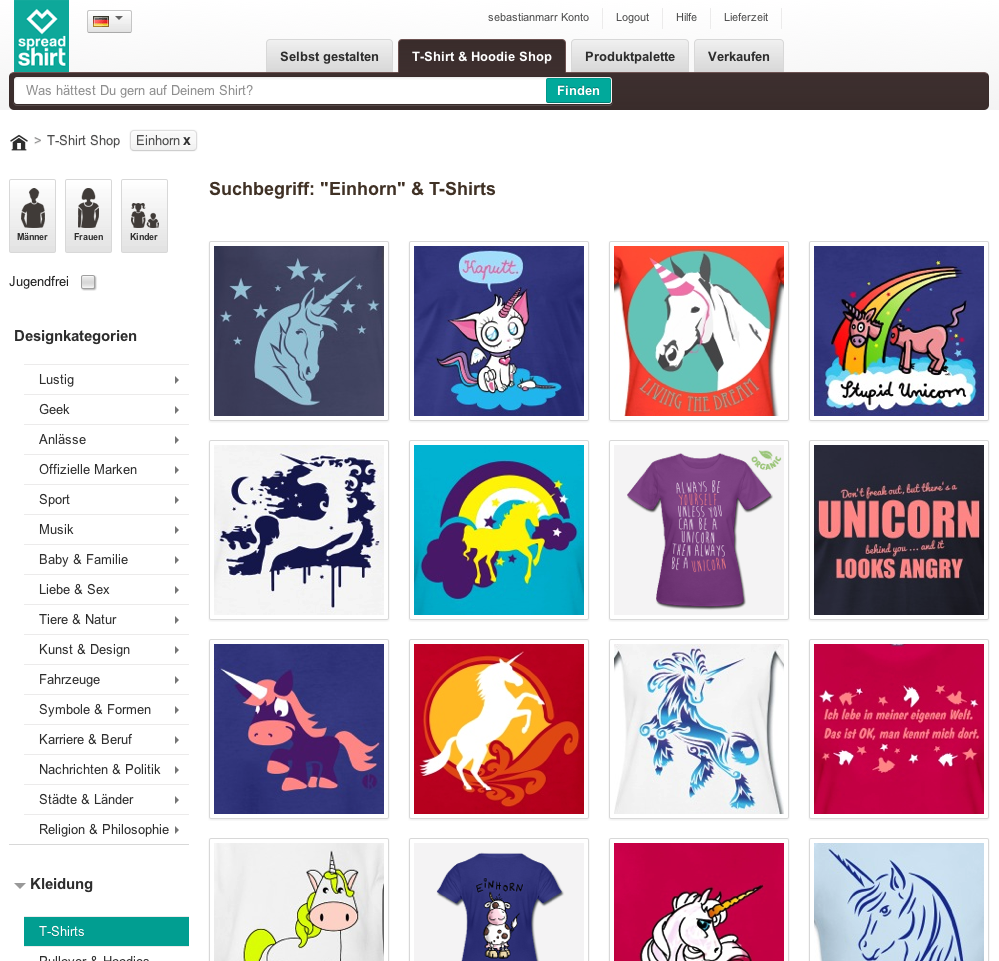
\includegraphics[width=0.9\textwidth]{search_result}
\caption{Suchergebnisseite}
\label{fig:search_result}
\end{figure}

Aufgrund der kürzlichen Einführung des Clicktracking-Systems wurde im Kontext dieser Arbeit mit den ersten \num{611836} aufgezeichneten Klicks gearbeitet.

\subsection{Datenqualität}

Die Qualität von Daten wird im Allgemeinen unter mehreren Gesichtspunkten beurteilt \cite{hkp2012}. Dazu gehören unter Anderem \emph{Korrektheit}, \emph{Vollständigkeit}, und \emph{Redundanzfreiheit}. Nachfolgend werden die bei Spreadshirt vorhandenen Daten nach diesen Kriterien betrachtet und die Quellen eventueller Fehler \cite[43 ff]{jo2003} diskutiert.

\paragraph{Korrektheit}

Die Korrektheit der Tag-Daten kann an vielen Punkten angezweifelt werden. Das hervorstechende Problem hierbei ist das Auftreten von Spam. Viele Partner versehen ihre Artikel und Designs mit Tags, die nicht den Inhalt beschreiben. Partner versehen ihre Designs und Artikeln mit falschen Tags, damit diese bei populären Suchbegriffen gefunden werden.

Ein weiterer Defekt ist die Inkorrektheit des Attributes \emph{Sprache} der Tags. Die Sprache wird aus der Domain abgeleitet, die der Benutzer, der den Tag eingegeben hat, besucht hat. Viele Partner geben jedoch ihre Tags in mehreren Sprachen ein, um ihre Inhalte besser auffindbar zu machen. Dies führt in der Konsequenz dazu, dass das Attribut Sprache im großen Teil der Tags als falsch angesehen werden kann.

Die Quelle beider Fehler ist also die bewusste Falscheingabe von Informationen, um einen persönlichen Vorteil zu erlangen.
                                                                                                                                                                                                                                                                                                                                                                                                              
\paragraph{Vollständigkeit}

Wie bereits in \ref{tag-system} beschrieben, fehlen in den Spreadshirt-Daten der Zeitpunkt und der Benutzer eines Taggings. Dies führt in der Konsequenz dazu, dass Spam schwerer erkannt werden kann. Zwar ist bekannt, wann ein Tag das erste Mal verwendet wurde, alle weiteren Verwendungen des Tags werden haben jedoch keinen Zeitstempel. Der Benutzer, der den Tag angelegt und verwendet hat, kann nur daraus abgeleitet werden, wer den getaggten Artikel angelegt hat.

Die Unvollständigkeit der Daten rührt in erster Linie daher, dass zum Zeitpunkt der Implementierung des Tag-Systems noch nicht bedacht wurde, dass die fehlenden Attribute später nützlich sein können.

\paragraph{Redundanzfreiheit}

Bedingt durch die Form der Dateneingabe besteht für das Vokabular des Tag-System ein großes Potential für redundante Daten. Da eingegebene Tags durch einen Separator getrennt eingegeben werden müssen, besteht hier Potential zur Fehleingabe. Wird der falsche Separator verwendet, werden die eigentlich getrennten Tags als eine einzige Entität abgespeichert.

Technisch kann jeder Tag genau ein Mal in der Datenbank vorkommen. Jedoch führen Rechtschreibfehler, unterschiedliche Groß- und Kleinschreibung, verschiedene Arten zusammengesetzte Wörter zu schreiben, Leerräume vor, nach und zwischen Wörtern eines Tags und Tippfehler dazu, dass das gleiche Wort mehrfach in der Datenbank gespeichert wurde.

Außerdem führten in der Vergangenheit Systemfehler und Implementierungsfehler dazu, dass falsche, nicht druckbare Zeichen in den Tags enthalten waren. Nach Beseitigung der Fehler blieben die fehlerhaften Tags bestehen, so dass bei einer erneuten Eingabe des gleichen Wortes ein neuer Tag in der Datenbank angelegt wurde.

\section{Lösungsansatz}

Die Beziehungen, die zwischen Wörtern und Wortgruppen hergestellt werden können, hängen stark von Umfang, Vielfältigkeit und Qualität der vorhandenen Datenquellen ab. Daher wurde zur Realisierung der Zielstellung ein iterativer Ansatz gewählt.

Die grundsätzliche Lösungsidee besteht in der Erstellung eines Graphen, dessen Knoten Wörter oder Wortgruppen darstellen. Die Kanten zwischen diesen Knoten repräsentieren inhaltliche Beziehungen. Ein erstrebenswertes Ziel ist also ein Graph mit möglichst vielen, duplikatfreien Knoten und vielen, nach inhaltlicher Nähe gewichteten, Kanten. Die hohe Knotenanzahl kommt zum Tragen, um möglichst alle Suchbegriffe und Themen des Anwendungsgebietes abzubilden. Kantenanzahl und -gewichte spielen dann eine Rolle, wenn nach den inhaltlich nächsten Nachbarn eines Knotens gesucht wird.

Um einen solchen Graphen zu erstellen, ist eine Grundmenge von Daten nötig. Diese Grundmenge stellen die Daten des Tag-Systems (\ref{tag-system}) von Spreadshirt dar. Die bereinigten Tags stellen die Knotenmenge dar. Die Kanten werden mittels Kookkurenz ermittelt.

Um die Qualität des Graphen danach schrittweise zu verbessern, werden daraufhin im Laufe der Arbeit weitere externe und interne Datenquellen integriert. Hierbei werden, soweit möglich, ebenfalls kookkurenzbasierte Ansätze gewählt. Diesem Vorgehen liegt die Annahme zu Grunde, dass oft gemeinsam auftauchende Begriffe auch eine inhaltliche Nähe zueinander aufweisen.

Bei jeder neuen Datenquelle muss zunächst die Bereinigung, Integration, Reduktion und Transformation der Daten durchgeführt werden \cite{hkp2012}. Diese Schritte gewährleisten die Datenqualität des Ergebnisgraphen.

Zusammengefasst bedeutet dies, dass abgeleitet von der vorhandenen Knotenmenge weitere Graphen aus anderen Datenquellen erstellt und diese dann in den ursprünglichen Graphen überführt werden. Dies führt einerseits unter Umständen zu einer Erweiterung der Knotenmenge und andererseits zu neuen Kanten mit neuen Gewichten.

Die gewichtete Kombination mehrerer Kanten zwischen zwei Knoten des Graphen stellt also im Ergebnis die inhaltliche Nähe der Begriffe dar, die durch die Knoten repräsentiert werden. Somit muss des weiteren eine geeignete Gewichtung der Kantentypen gefunden werden. Dies ist aufgrund der Natur des Problems nur mit Hilfe von menschlicher Bewertung möglich. Diese Optimierung kann somit gleichzeitig mit der Evaluation statt finden.

Um den Lösungsansatz technisch umzusetzen, soll wenn möglich das Programmiermodell MapReduce \cite{dg2004} eingesetzt werden, da dieses die Skalierung des Vorgehens auf beliebige Datenmengen ermöglicht. Speziell die Erstellung von Kookkurenzgraphen kann deutlich von der Verwendung dieses Verfahrens profitieren.

In den nachfolgenden Kapiteln werden die Umsetzung dieses Lösungsansatzes und die Ergebnisse detailliert beschrieben.